\documentclass[letterpaper,headings=standardclasses]{scrartcl}

\usepackage[margin=1in,includefoot]{geometry}
\usepackage{amssymb}
\usepackage{amsmath}
\usepackage{listings}
\usepackage{tikz}
\usepackage{float}

\usetikzlibrary{shapes,arrows}

\tikzset{
  block/.style    = {draw, thick, rectangle, minimum height = 3em, minimum width = 3em},
  sum/.style      = {draw, circle, node distance = 2cm},
  input/.style    = {coordinate, circle},
  output/.style   = {coordinate, circle}
}

\lstset{basicstyle=\ttfamily,columns=flexible,breaklines=true}

\title{Homework 1}
\subtitle{CS 559 - Neural Networks - Fall 2019}
\author{Matteo Corain 650088272}

\begin{document}

\maketitle

\section{Question 1}

In order to design a network that implements the given function using the signum activation function, it has been decided to follow the standard design procedure for the first layer of neurons (i.e. using a single neuron for each logical product) and to design a custom second layer (made up of a single neuron) to implement a modified OR logical function.

\subsection{First logical product}

For the implementation of the first logical product $\bar{x_1} x_2 x_3$, the standard design process has been followed. Using the presented nomenclature, we have:

$$ n = 1 $$
$$ m = 2 $$

Therefore, a possible choice of weights that implements the requested logical function is:

$$ w_0 = -m + \frac{1}{2} = -\frac{3}{2} $$
$$ w_1 = -1 $$
$$ w_2 = w_3 = 1 $$

\subsection{Second logical product}

The same process has been followed also for the implementation of the second logical product $ x_1 \bar{x_2} $; given that input $x_3$ does not appear in this formulation, a possible choice of weights that implements the requested logical function is:

$$ w_0 = -m + \frac{1}{2} = -\frac{1}{2} $$
$$ w_1 = 1 $$
$$ w_2 = -1 $$
$$ w_3 = 0 $$

\subsection{OR logical function}

For the implementation of the OR logical function, a custom design has been necessary since the two neurons in the first layer do not output, as usual, value 0 in case of false, but instead they output value -1. The single neuron in the second layer of the network, therefore, has to implement the logic function described by the following truth table:

\begin{table}[H]
\centering
\begin{tabular}{|c|c|c|}
\hline
$x_1$ & $x_2$ & $y$  \\ \hline
-1    & -1    & -1   \\ \hline
-1    & 1     & 1    \\ \hline
1     & -1    & 1    \\ \hline
1     & 1     & 1    \\ \hline
\end{tabular}
\caption{Truth table for the OR logical function using signum activation}
\end{table}

There are different approaches that can be followed for designing a neuron that implements this logic function. One of the simplest is a graphical procedure, as described in the following. If we plot the $x_1$-$x_2$ plane, we can see that the data points belonging to the two classes, yielding values -1 and 1, are clearly linearly separable. One of the possible lines that separate the two classes, as shown in the figure, satisfies the relation:

$$ 1 + x_1 + x_2 = 0 $$

\begin{figure}[H]
\centering
\includegraphics[width=.75\linewidth]{or_func.pdf}
\caption{Data plane for the OR logical function using signum activation}
\end{figure}

Remembering the general equation of a linear separator in a perceptron ($ w_0 + w_1x_1 + w_2x_2 = 0 $), a possible choice of weights that can be used to implement such a separator is:

$$ w_0 = w_1 = w_2 = 1 $$

This may also be analytically verified if we write the system of linear inequalities that describe this logical function; in fact, from the truth table we have that:

$$ \begin{cases} \text{sgn(} w_0 - w_1 - w_2 \text{)} = -1 \\ \text{sgn(} w_0 - w_1 + w_2 \text{)} = 1 \\ \text{sgn(} w_0 + w_1 - w_2 \text{)} = 1 \\ \text{sgn(} w_0 + w_1 + w_2 \text{)} = 1 \end{cases} \Rightarrow \begin{cases} w_0 - w_1 - w_2 < 0 \\ w_0 - w_1 + w_2 > 0 \\ w_0 + w_1 - w_2 > 0 \\ w_0 + w_1 + w_2 > 0 \end{cases} $$

It is simple to verify that the identified weights satisfy the four identified inequalities.

\subsection{Final network}

A possible network that implements the logical function $f(x_1,x_2,x_3) = \bar{x_1} x_2 x_3 + x_1 \bar{x_2}$, using the previously computed weights, is depicted in the figure below.

\begin{figure}[H]
\centering
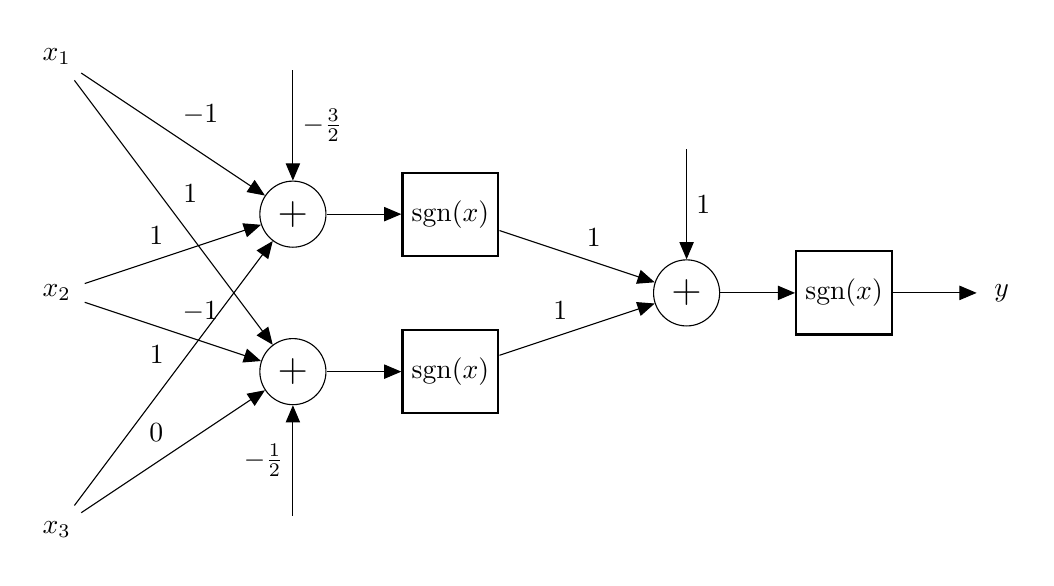
\begin{tikzpicture}[auto, node distance=2cm, >=triangle 45]

% Input layer
\draw node [input, name=x1] {$x_1$};
\draw node [input, name=x2, below of=x1, node distance=3cm] {$x_2$};
\draw node [input, name=x3, below of=x2, node distance=3cm] {$x_3$};

% First layer
\draw node [sum, right of=x2, yshift=1cm, node distance=3cm] (sum1) {\Large$+$};
\draw node [sum, below of=sum1] (sum2) {\Large$+$};
\draw node [input, name=x01, above of=sum1] {};
\draw node [input, name=x02, below of=sum2] {};
\draw node [block, right of=sum1] (act1) {sgn($x$)};
\draw node [block, right of=sum2] (act2) {sgn($x$)};

% Second layer
\draw node [sum, right of=act1, yshift=-1cm, node distance=3cm] (sum3) {\Large$+$};
\draw node [input, name=x03, above of=sum3] {};
\draw node [block, right of=sum3] (act3) {sgn($x$)};
\draw node [output, name=y, right of=act3] {$y$};

% Connections
\draw[->](x01) -- node {$-\frac{3}{2}$}(sum1);
\draw[->](x1) -- node {$-1$}(sum1);
\draw[->](x2) -- node {$1$}(sum1);
\draw[->](x3) -- node {$1$}(sum1);
\draw[->](x02) -- node {$-\frac{1}{2}$}(sum2);
\draw[->](x1) -- node {$1$}(sum2);
\draw[->](x2) -- node {$-1$}(sum2);
\draw[->](x3) -- node {$0$}(sum2);
\draw[->](sum1) -- node {}(act1);
\draw[->](sum2) -- node {}(act2);
\draw[->](x03) -- node {$1$}(sum3);
\draw[->](act1) -- node {$1$}(sum3);
\draw[->](act2) -- node {$1$}(sum3);
\draw[->](sum3) -- node {}(act3);
\draw[->](act3) -- node {}(y);

\end{tikzpicture}
\caption{Final network that implements the given function}
\end{figure}

\section{Question 2}



\section{Question 3}

\subsection{Complete Python code}

\lstinputlisting[basicstyle=\ttfamily\scriptsize,language=python]{hw1_ex3.py}

\end{document}